\documentclass[10pt,oneside,a4paper,final,english]{memoir}

\usepackage{palatino}
\usepackage{microtype}
\usepackage{lscape}
\usepackage{multicol}
%\usepackage{epic,eepic}
\usepackage{latexsym}
\usepackage{verbatim}
\usepackage{listings}
\usepackage{ulem}
\usepackage{hyperref}

\let\footruleskip\undefined
\usepackage{fancyhdr}
\usepackage[final]{fixme}

\let\fref\undefined
\usepackage[plain]{fancyref}

%% FOR LOOP
\usepackage{ifthen,calc}
\newcounter{myforloopcounter}
\newcommand{\forloop}[5][1]% 
{\setcounter{#2}{#3}% 
\ifthenelse{#4}% 
{#5%
  \addtocounter{#2}{#1}% 
  \forloop[#1]{#2}{\value{#2}}{#4}{#5}% 
}%
% Else 
{}%
}% 


%% USAGE
%\forloop[step]{counter}{initial_value}{conditional}{code_block} 
\usepackage[english]{babel}
\usepackage[utf8]{inputenc}

%\selectlanguage{danish}

\lstset{language=Python,basicstyle=\small,
  columns=fullflexible}


\usepackage[pdftex]{graphicx}

\DeclareGraphicsExtensions{.jpg .png .pdf}


\usepackage{amsmath}
\usepackage{latexsym}
\usepackage{amssymb}


\usepackage[osf,sc]{mathpazo}
\usepackage{microtype}
%\usepackage{fourier}
\linespread{1.05}

%\usepackage[charter]{mathdesign}
%\usepackage{lmodern}

%\usepackage{algorithmic}
%\usepackage{algorithm}

\usepackage{amsthm}


\theoremstyle{plain}  \newtheorem{definition}{Definition}
\theoremstyle{remark} \newtheorem{lemma}{Lemma}
\theoremstyle{plain}  \newtheorem{theorem}{Theorem}
\theoremstyle{remark}  \newtheorem{example}{Example}


\newcommand{\p}{\ensuremath{^\prime}}
\DeclareGraphicsExtensions{.jpg, .eps, .png}
%%% Local Variables:
%%% mode: plain-tex
%%% TeX-master: "../master"
%%% End:

\usepackage{algorithmic}
\usepackage{algorithm}
\usepackage[sectionbib,square]{natbib}
%\bibpunct{(}{)}{,}{a}{}{}
\setcitestyle{alpha}
%\setcitestyle{numbers,aysep={},yysep={;}}

\usepackage{datetime}

\chapterstyle{thatcher}

%\pagestyle{fancy}
\begin{document}
  \fontencoding{T1}
%  \fontseries{m}
%  \fontshape{n}
%  \fontsize{12}{15}
%  \selectfont


%%%%%%%%%%%%%%%%%%%%%%%%%%%%%%%%%%%%%%%%%%%%%%%%%%%%%%%%
%                    Forside
%%%%%%%%%%%%%%%%%%%%%%%%%%%%%%%%%%%%%%%%%%%%%%%%%%%%%%%%
\makeatletter % open mode for reading @ signed variables
\def\maketitle{%
 \null
 \thispagestyle{empty}%
 \vfill
 \begin{center}\leavevmode
   \normalfont
   \LARGE{\raggedleft \@title\par}%
   \hrulefill\par
   \large{\raggedleft \subtitle\par}%
   \vskip 2cm
   {\today\par}%
 \end{center}%
 \vfill
 \begin{flushleft}
   {\large \@author } \\
   {\footnotesize \suplementInfo }
 \end{flushleft}
 \clearpage % Terminates the page here. Everything else vil be placed
            % on next page.
}
\makeatother % closing mode for reading @ signed variables
%%%%%%%%%%%%%%%%%%%%%%%%%%%%%%%%%%%%%%%%%%%%%%%%%%%%%%%%
%               Data til forside
%%%%%%%%%%%%%%%%%%%%%%%%%%%%%%%%%%%%%%%%%%%%%%%%%%%%%%%%
\title{Final Hand In $\cdot$ Week VIII}

\def\subtitle{CCO $\cdot$ Constraint Continuous Optimization}

\author{Johan Sejr Brinch Nielsen} \def\suplementInfo{

\kern 5pt \hrule width 11pc \kern 5pt

\begin{tabular}{ll}
Email: & zerrez@diku.dk  \\
Cpr.:  & 260886-2547
\end{tabular}

% putter 5pt spacing oven over og neden under stregen
\kern 5pt \hrule width 11pc \kern 5pt

Dept. of Computer Science,  \\
University of Copenhagen

}


\maketitle
\newpage


\section{Introduction}
This task consists of finding three angles that together will move an
``arm'' to some specified point in the 2D-plane. Specifically, one
must optimize the angles using Newton's method to get a good
approximation of the angles needed.


\section*{A: End-Effector Function}
A homegenous transformation works by multiplying $n$ matrices (one for
each connecting angle) with a point, like so: $T_0T_1T_2 \ldots T_n
\cdot p$ \\
Where the $i$th tranformation matrix $T_i$ represents the $i$th angle
and $p$ is the point that needs transformation.

Each matrix will rotate the intermediate point with matrices
associated angle and tanslate the point with the associated length.

The point $p$ needs to be expanded with an extra ``dimension'' to make the math
work (watch out; it's a trick). \\

The transformation function $f$ now becomes: \\
$f(\theta^n) = T_1T_2T_3 \ldots T_n \cdot x^d$ \\
Where $\theta^n$ is the $n$ dimensional angle vector and $x$ is the
$d$ dimensional point to transform. If the cartesian coordinates were
$(1,2,3)$ then the homegenous coordiate becomes $(1,2,3,1)$.\\

In our particular case (with just 2 dimensions and 3 angles) the
transformation function $f$ becomes:\\
$f(\theta^3) = T_1T_2T_3 \cdot x^2$\\
Where $x$ is the $2$-dimensional point.

In $2$ dimensions the transformation matrix $i$ becomes:
\[ \left|
  \begin{array}{ccc}
    \cos\theta_i & -\sin\theta_i & x_i \\
    \sin\theta_i & \cos\theta_i & y_i \\
    0 & 0 & 1
  \end{array}
\right| \]


\section*{B: Derivate of the End-Effector}
The End-Effector is the resulting point after the transformation
described above. This can be expressed as a vector parameterized by
the angles by multiplying the starting point to the transformation
matrices. The task is to get the end effector as close the goal as
possible.

The resulting term describing the end effector will consist of
addition of $\sin/\cos$ and constant terms. The derivative can be
easily computed by computing this for each of the different variables
(the angles).

\section*{C: Root Search Problem}
The initial guess $\theta^3$ yields the first end effector by:
\[ e = f(\theta^3) \]

Denote the difference between the goal $g$ and the end effector $e$ by
$\Delta\theta$. The goal is now to find the root of $\Delta\theta$,
hence the problem is that of a root-search.


\section*{D: Nonlinear Newton Method}
We need to find a good guess on $\Delta\theta$ such that:
\begin{center}
$g' = f(\theta + \Delta\theta)$ is closer to $g$ than $f(\theta)$.
\end{center}

A simple guess is to look at the first Tayler expansion:
\[ g' = f(\theta_0) + \frac{\delta
  f(\theta_0)}{\delta\theta_0}\Delta\theta \]
With a rest of $O(\mid\mid \Delta\theta^2\mid\mid)$. \\

Letting,
\[\theta_{i+1} = \theta_i +
\frac{\delta f(\theta_i)}{\delta\theta_i}\Delta\theta_i \]
should yield a better guess than the $\theta_i$. This method
approximates the goal in a linear way, always leaving a
rest. Hopefully the rest, hence the distance to the goal, will close
in on zero.



\section*{Implementation}

\subsection*{Pseudo Code}
Here are the pseudo code for the root finder:
\begin{verbatim}
ik-solver(t0, g, e)
 t = t0
 e = f(t)
 while( |g-e| > e) do
  dt = j_0^-1(g-e)
  t  = t + dt
  e  = f(t)
 end while
 return dt
end
\end{verbatim}

\subsection*{Nonlinear Newton}
This is my implementation of the nonlinear Newton's method. As can be
seen, the implementation always runs for 20 rounds (this could be
replaced by an error meassure):
\begin{verbatim}
function [ angles ] = nonlinear_newton( g, t, angles )
%
% input
%     g      : Goal position/vector (specified in homogenuous coordinates)
%     t      : A vector of fixed rod-link vectors
%     angles : A vector with joint angles
%     e      : Position/vector (specified in homogenuous coordinates)
% output
%     angles : The updated pose which will reach the specified goal position.

e  = [0;0;1];
ep = f(t, angles);

for i=1:20
    da = pinv(jacobian(t, angles, e))*(g - ep);
    angles = angles + da;
    ep = f(t, angles);
end

end
\end{verbatim}

\subsection*{F-function}
This is my implementation of the $f$ function:
\begin{verbatim}
function [ e ] = f( t, angles, e )
% F The end-effector function
%   Given an initial configuration of a inverse kinematics chain
%   with a root fixed at the origin this function computes
%   the x-y position of the end-effector.
% input
%     t      : A vector of fixed rod-link vectors
%     angles : A vector with joint angles
%     e      : Position/vector (specified in homogenuous coordinates)
% output
%     e : The end-effector position/vector given in root frame
if nargin < 3
  e = [0.0;  0.0; 1.0];
end

% Generate transformation matrices
for i=1:length(angles)
    j = length(angles)-i+1;
    angle = angles(j);
    m = [
        cos(angle), -sin(angle), t(1,j);
        sin(angle), cos(angle),  t(2,j);
        0, 0, 1
        ];
    e = m * e;
end

if( ~isequal(e(3),0))
    e = e./e(3);
end
end
\end{verbatim}


\subsection*{Verification of Implementation}
I have tested the implementation briefly, by picking out some points
at random. The results seems correct:\\
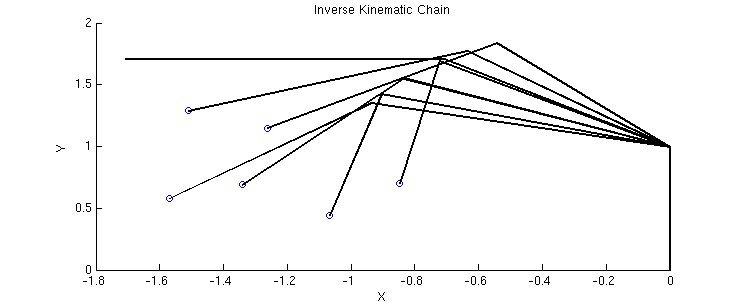
\includegraphics[scale=.7]{shot.png}

The image suggests that the code works correctly, since the arms are
touching the points i chose. There can however exist points (example
out of reach of the arm) that I have not tested due to time
limitations.



\end{document}

%%% Local Variables:
%%% mode: latex
%%% TeX-master: t
%%% End:
